\chapter{Introduction}\label{chap:introduction}
 Climate change leads to higher average and daily maximum temperatures as well as a more frequent occurrence of heat waves \citep{meteoschweiz_klimaindikatoren_2024, ipcc_2023}. For example, summers in Switzerland during 2023, 2022, 2019, 2018, 2017, and 2015 have demonstrated a marked increase in the frequency of prolonged periods of high temperatures \citep{heatwaves_switzerland}. Figure~\ref{fig:number_of_hot_days} depicts this trend.

  \begin{figure}[H]
    \centering
    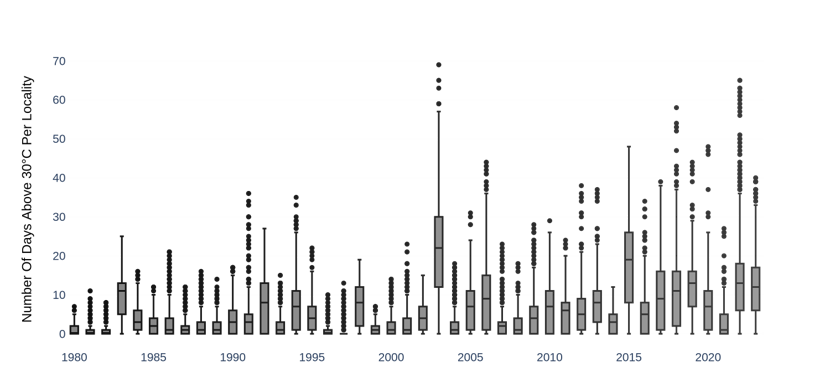
\includegraphics[width=\textwidth]{thesis/figures/number_of_hot_days_switzerland.png}
    \caption{Annual frequency distribution of hot days in all localities within Switzerland since 1980, where a hot day is characterized by a maximum temperature exceeding 30°C.}
    \label{fig:number_of_hot_days}
\end{figure}
 
 These unfavorable weather conditions are detrimental to agricultural production. For dairy farmers, elevated temperatures can adversely affect milk yield, quality, fertility, and other related factors \citep{bernabucci_effect_2015,lambertz_climatic_2014, bohmanova_temperature-humidity_2007, dunn_analysis_2014,ranjitkar_will_2020, west_effects_2003, gantner_differences_2017,maggiolino_estimation_2020,salfer_annual_2019,smith_short_2013,hammami_evaluation_2013,hill_dairy_2015, vitali_effect_2015, cox_mortality_2016}. 
 The magnitude of the effects of heat stress on dairy milk production varies across breeds and has been analyzed for a subset of breeds and geographic regions outside of Switzerland \citep{bryant_quantifying_2007, smith_short_2013, gantner_differences_2017, ahmed_temperature_2022}. Although the dairy sector represents the largest share of the national agricultural production, accounting for 23\% of total output with over 545'000 cows \citep{agrarbericht_2023}, the extent to which dairy producers are exposed to quantitative and qualitative milk losses for different breeds remains uncertain. According to the Swiss Federal Office of Agriculture the agricultural production should be adapted to climate and regional properties. In line with this objective, this work provides an assessment on how hot weather impacts the milk quantity and quality in Switzerland. In particular, we examine how milk yield (MY) and energy-corrected milk yield (ECM) are affected by varying levels of the Temperature Humidity Index (THI). Acknowledging that previous studies indicate diverse coping mechanisms with heat stress among breeds, this research emphasizes a comparative analysis of multiple breeds. To facilitate this investigation, we utilize subsamples from a dataset comprising 130 million test-day samples sourced from the three principal breeding organizations in Switzerland. These samples span a period of 42 years, from 1982 to 2023, with data from six predominant breeds: Holstein, Brown Swiss, Original Braunvieh, Swiss Fleckvieh, Simmental, and Jersey. The dataset covers the entire national territory.



\section{Literature Review}
\paragraph{The Effect of Heat Stress Across Dairy Cow Breeds} \quad \\
\textit{Different breeds have different responses to heat stress with respect to milk production. The impact of heat stress while making a distinction between breeds is globally understudied.}

The majority of studies assessing the impact of heat stress on the performance of dairy cows focus on a single breed, with examples such as \cite{bernabucci_effect_2015, lambertz_climatic_2014,hammami_evaluation_2013, hill_dairy_2015}. Only a limited number of authors consider multiple breeds. According to \cite{bryant_quantifying_2007}, Holstein Friesians exhibit greater sensitivity to heat effects compared to New Zealand Jerseys, with the latter maintaining a more stable milk yield under elevated 3-day mean THI conditions. No significant differences were observed in protein and fat content between the two breeds. \cite{smith_short_2013} report an increase in milk production among Jersey cows during heat stress, while performance declines for Holsteins in a research farm in the United States. \cite{gantner_differences_2017} explore the milk performance of Holstein and Simmental cows in Croatia, finding a greater vulnerability to heat stress among high-producing cows compared to their low-performing counterparts. Their findings suggest a higher resistance to heat stress in Simmental breeds compared to Holsteins, though further research is warranted. \cite{ahmed_temperature_2022} examine the effects of heat shocks—defined as periods of five consecutive days with average temperatures exceeding 25°C—on milk production. Overall, no significant differences in heat shock tolerance were observed among Swedish Holsteins, Swedish Reds, and a crossbreed of the two in Sweden, suggesting that breed diversification as a strategy to mitigate heat stress risks is ineffective. Nonetheless, Swedish Red cows exhibit greater resilience to negative heat effects when considering heat events in relation to the genetic milk index. \cite{cuellar_differences_2023} include Brown Swiss in a comparative study with Holsteins and their crossbreeds, finding a more pronounced decrease in milk yield for Brown Swiss than for Holstein. 

\paragraph{The Effect of Heat Stress in Swiss Dairy Production} \quad \\
\textit{The effect of heat stress on the quantity and quality of milk production at the animal-level for commercial farms in grassland-based systems over a long period of time is understudied in Switzerland.}

Globally, the phenomenon of heat stress in dairy cows is extensively researched, particularly at the level of individual animals in research farms. Additionally, numerous studies have quantified the effects of heat stress on dairy cows using panel data across various regions worldwide. The works mentioned in the preceding paragraph represent only a select number of these investigations. Only a few recent studies consider data from Switzerland to study the effects of heat stress on dairy cows: \cite{bucheli_heat_2022} analyze the annualized farm-level effect of heat stress on milk revenues, veterinary expenses and feed purchases. In the period from 2003 to 2015 Swiss farmers are on average financially robust to heat exposure. However, this does not imply non-existence of a related risk. \cite{gasser_can_2023} find that meteorological features do not improve the accuracy of daily milk yield predictions. The data originates from an experimental farm in Tänikon, Switzerland. Furthermore, \cite{holinger_behavioural_2024} observe behavioral changes in cows under heat stress with data of four Swiss commercial farms in the period from June to September 2021. During days characterized by elevated maximum THI values, cows are observed more frequently in proximity to the drinker during the morning hours. In contrast, during the afternoon, they tend to congregate in close proximity to each other and seek shade. Moreover, on such days, there is a notable decrease in the duration of time spent lying down, accompanied by an increase in their locomotor activity as noon approaches.

\section{Research Objective}
This study seeks to build upon methodologies established in prior research to examine the impact of heat stress on Swiss dairy production across various breeds. Although the complex physiological responses of individual animals to heat stress are extensively studied and well documented \citep{kadzere_heat_2002,becker_invited_2020}, the effects of heat stress at broader geospatial scales, including herd, regional, and national levels in grassland-based systems across breeds, remain under-researched. Swiss dairy farms predominantly employ pasture-based systems, with cows spending substantial amounts of time grazing outdoors \citep{agrarbericht_2023}. Evaluating the effects of THI on milk performance variables within this production context could provide valuable insights into the actual influence of ambient temperature and humidity on dairy cows.

\vspace*{\baselineskip}
Heat stress exerts a direct impact on economically significant factors, including milk yield, milk component yield, and the health of cows. For dairy farmers, variations in the quantity and quality of production are anticipated and regarded as standard to some degree. Nevertheless, these agronomic factors are intrinsically connected to the dairy producers' revenue streams from milk. Farmers continuously modify their management practices, generally through technological advancements, enhanced knowledge, or shifts in policy \citep{agrarbericht_2023, koutouzidou_evolution_2022}, as well as in response to heat stress \citep{ji_review_2020,vroege_effects_2023}. This includes, for example, feeding regimes, housing systems, cooling systems, milking technologies or breeding strategies \citep{kadzere_heat_2002, west_effects_2003}. All these potentially confound heat stress effects and pose obstacles for a full isolation of the causal weather effects.

\vspace*{\baselineskip}
Switzerland is a topologically diverse country. This geographic variability leads to different heat exposures on a regional level as depicted on Figure~\ref{fig:thi_80}. The effective animal-level heat exposure depends on many environmental factors. In our work, our aim is to develop a framework to isolate the weather effects from farm-specific properties, spatial heterogeneity, herd characteristics, as well as individual animal responses and assess their impact on the aforementioned agronomic indicators. Moreover, we specifically check for weather effect differences across breeds to validate if certain breeds are more-heat stress tolerant than others and may qualify for heat-stress resilience under the warming climatic trends in Switzerland. Our analysis remains at the breed level and does not consider genomic selection or herd evolution.

\begin{figure}[H]
    \centering
    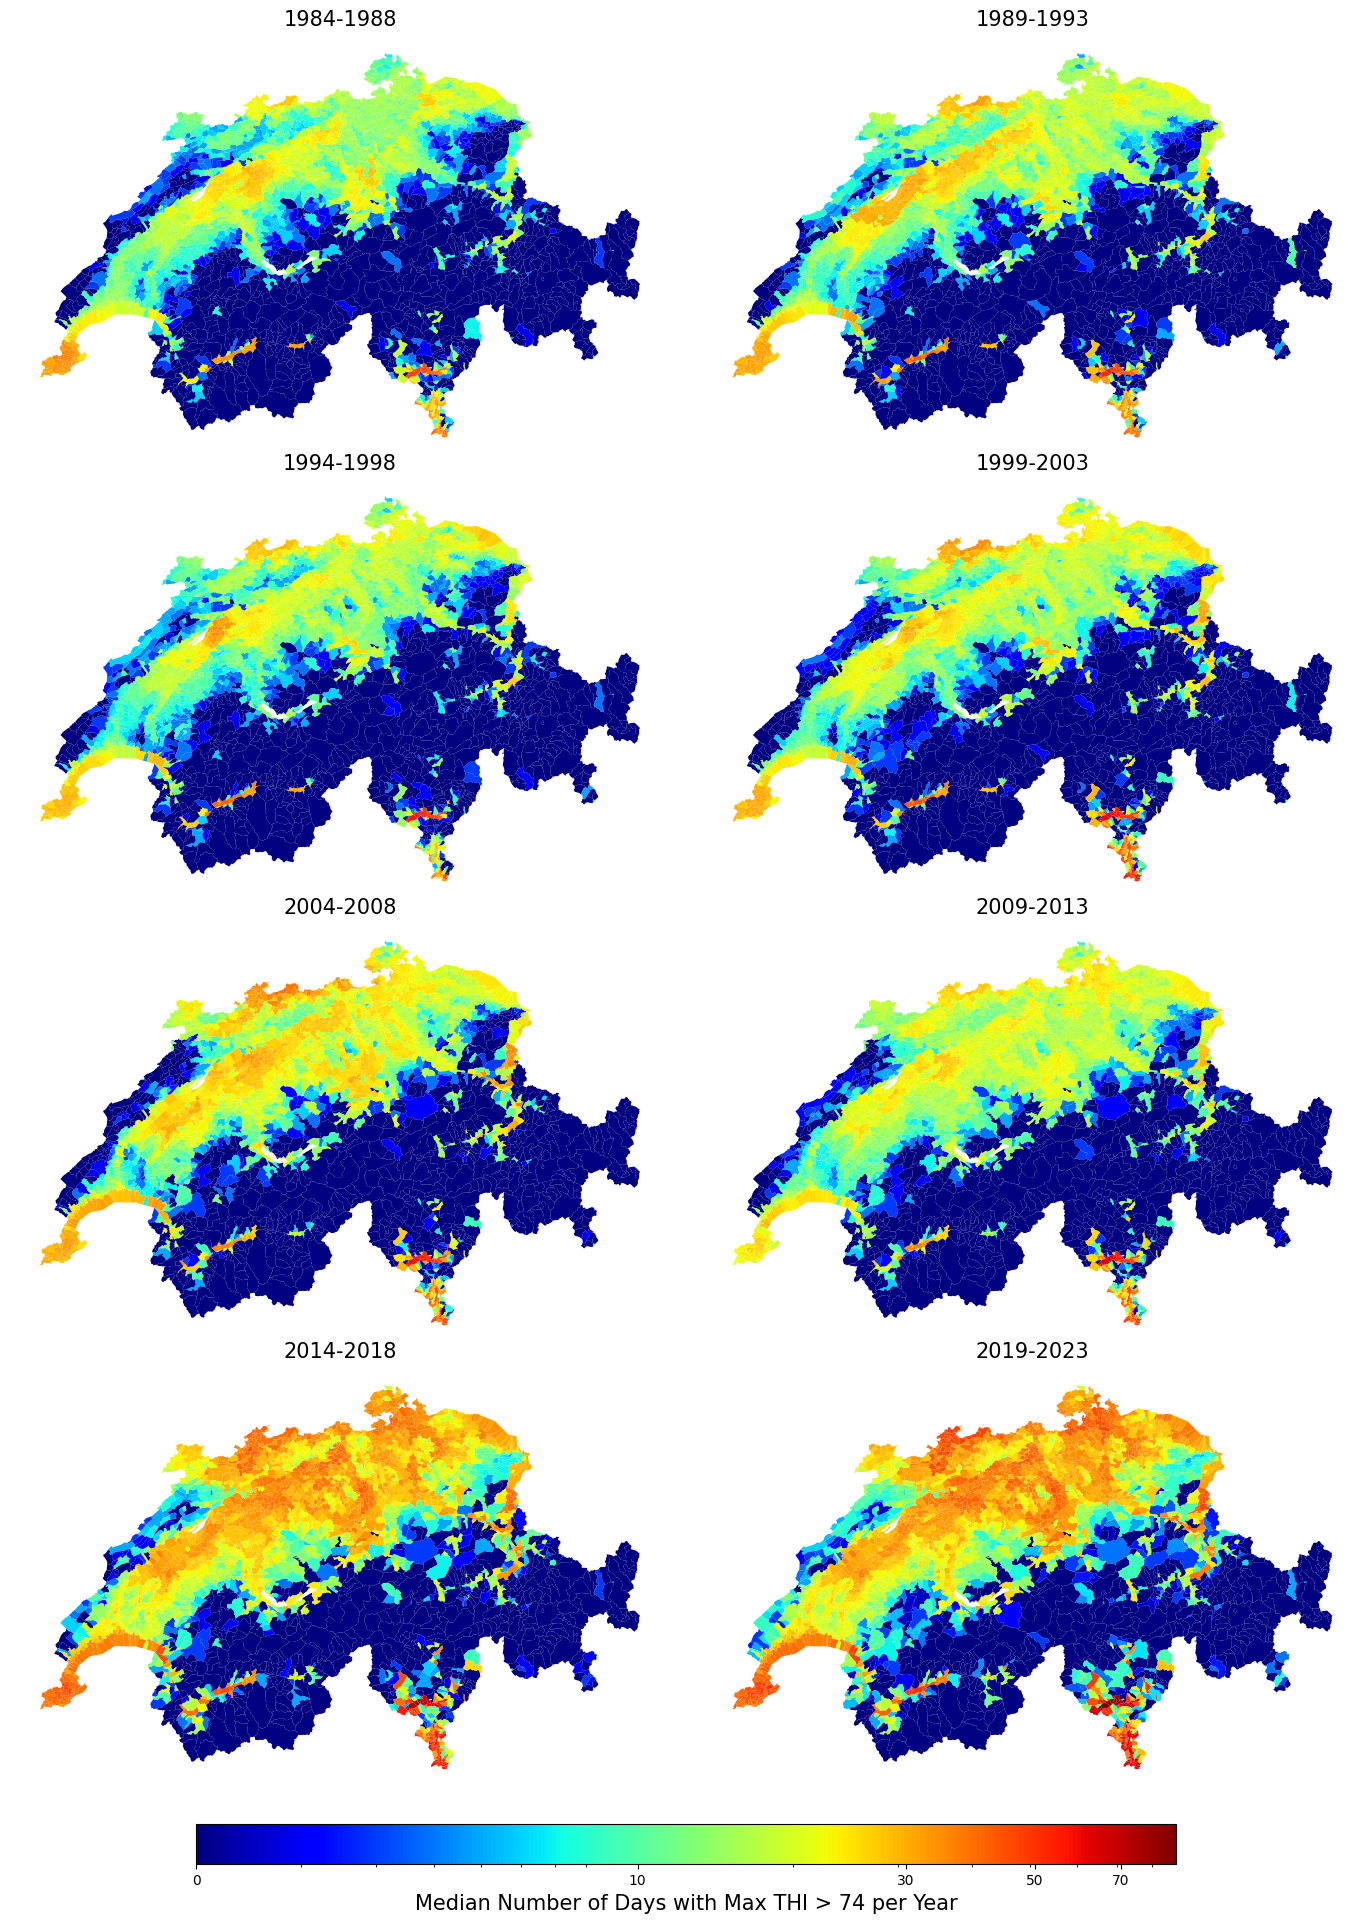
\includegraphics[width=\textwidth]{figures/00_thi_above_80/thi_above_74.png}
    \caption{The median number of days when the maximum THI surpasses the threshold 74 substantially increases for some regions in the period $t_1$ from 1984 to 2023. A THI of 74 stands for moderate heat stress. The coloring scheme is logarithmic because some towns in the canton Ticino (southermost part) exceed the median compared to the rest of Switzerland considerably. Moreover, dairy farming is more widespread in the northern parts of Switzerland.}
    \label{fig:thi_80}
\end{figure}

\section{Research Question and Hypothesis}\label{sec:research_question}
To achieve the above-mentioned objective, the study sets the main focus on the following research question:

\begin{center}
    \textit{At what Temperature Humidity Index (THI) values do changes in dairy performance occur for the different dairy cow breeds in Switzerland?}
\end{center}

The primary variables under consideration are the milk yield, measured in kilograms per day, and the energy-corrected milk yield (ECM), also measured in kilograms per day. The ECM incorporates yields from both fat and protein components. Recognizing the variance in component yields across different breeds, the ECM yield provides a standardized measure for comparative analysis among breeds. Building upon previous studies, it is anticipated that both volumetric and component yields will decline once specific thresholds of the Temperature-Humidity Index (THI) are surpassed. Reported threshold values include 68 \citep{de_rensis_seasonal_2015}, 72 \citep{armstrong_heat_1994}, and 76 \citep{vroege_effects_2023}\footnote{Many studies employ differing definitions of THI and utilize diverse aggregation methodologies, including summation, averaging, as well as determining minimal or maximal values over hours, single days, multiple days, weeks, months, or even years. Consequently, careful consideration is imperative in the interpretation of THI values.}. It is further anticipated that there will be breed-specific variations in the THI values critical for optimal dairy performance \citep{kadzere_heat_2002}. Jerseys are posited to exhibit greater heat tolerance compared to Holsteins, a characteristic also expected in the Simmental breed. In conclusion, the Holstein breed, known for high yields, is likely to experience greater stress under increased heat conditions compared to lower-yielding breeds such as Simmental and Jersey.

\section{Organization}
The remainder of this document is organized as follows: First, in Chapter~\ref{chap:background}, we provide an overview of various aspects regarding heat stress in dairy cows, breeds, and farms to set the agronomic scope. This includes aspects from animal physiology, but also political and economic aspects of the Swiss dairy market because our study covers a time period of 42 years. Second, within Chapter~\ref{chap:material_methods}, in consideration of the non-experimental nature of our study, we delineate our data strategy along with an exploratory data analysis in Section~\ref{sec:data}. This examination incorporates the agronomic, the meteorological, and the geospatial data. Guided by our research question and the insights gained from the data analysis, we determine the appropriate model and estimation strategy in Section~\ref{sec:models} and Section~\ref{sec:estimating_gams}. This includes our methodological advancement to estimate Generalized Additive Mixed Models with an unprecedented number of random effect factor levels. Third, we analyze and discuss the findings in Chapter~\ref{chap:results}. The concluding Chapter~\ref{chap:conclusion} summarizes our contributions, limitations, and also proposes future research directions.